% begin module implicit-tangent-line
\abovedisplayskip=0pt
\belowdisplayskip=0pt
\abovedisplayshortskip=0pt
\belowdisplayshortskip=0pt
\begin{frame}
\begin{example}
Find an equation of the tangent line to $(x-1)^2 + (y+2)^2 = 25$ at $(-2,2)$.
\begin{columns}
\column{1.2in}
\begin{center}
\only<handout:0|-15>{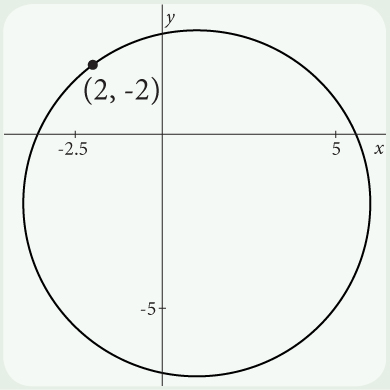
\includegraphics[height=3cm]{implicit-differentiation/pictures/implicit-tangent-linea.jpg}}
\only<16->{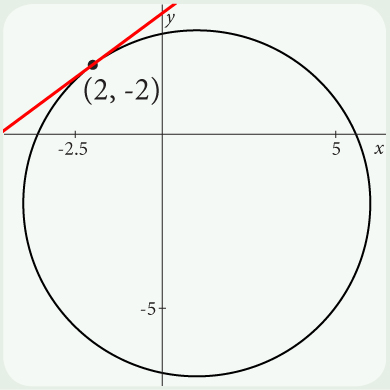
\includegraphics[height=3cm]{implicit-differentiation/pictures/implicit-tangent-lineb.jpg}}
\end{center}
\begin{align*}
\uncover<15->{&\text{Plug in} \ (-2,2):}\\
\uncover<15->{&\frac{\diff y}{\diff x}  = \frac{1+2}{4} = \frac{3}{4}}\\
\uncover<16->{&\text{Point-slope form:}\\
&y-2 = \frac{3}{4} (x+2)}
\end{align*}
\column{3in}
\abovedisplayskip=0pt
\belowdisplayskip=0pt
\abovedisplayshortskip=0pt
\belowdisplayshortskip=0pt
\begin{align*}
\uncover<2->{\text{Find} \ \frac{\diff y}{\diff x}, \ \text{given} \ (x-1)^2 \ + (y+2)^2 & = 25:} \\
\uncover<3->{\alert<handout:0|3-4>{\frac{\diff}{\diff x}\left((x-1)^2\right)} + \alert<handout:0|5-6>{\frac{\diff}{\diff x}\left((y+2)^2\right)}   &= \alert<handout:0|7-8>{\frac{\diff}{\diff x}(25)}}\\
\uncover<3->{\uncover<4->{\alert<handout:0|4>{2(x-1)\alert<handout:0|9>{\frac{\diff}{\diff x}(x-1)}}} +\uncover<6->{\alert<handout:0|6>{ 2(y+2)\alert<handout:0|11-12>{\frac{\diff}{\diff x}(y+2) }}}  &= \uncover<8->{\alert<handout:0|8>{0}}}\\
\uncover<9->{2(x-1)\alert<handout:0|9-10> {(\uncover<10->{1})}+ 2(y+2)\alert<handout:0|11-12>{\left( \uncover<12->{\frac{\diff y}{\diff x}} \right)}  & = 0}\\
\uncover<13->{2(y+2)\left( \frac{\diff y}{\diff x} \right) & = -2(x-1)}\\
\uncover<14->{\frac{\diff y}{\diff x} &=  \frac{1-x}{y+2}}
\end{align*}
\end{columns}
\end{example}
\end{frame}
% end module implicit-tangent-line